\documentclass[14pt,titlepage]{extarticle}
\usepackage{ucs}
\usepackage[utf8x]{inputenc}
\usepackage[english,russian]{babel}
\usepackage{indentfirst}
\usepackage[usenames,dvipsnames]{color}
\usepackage{algorithm}
\usepackage{algorithmic}
\usepackage[pdftex]{graphicx}
\usepackage{multicol}


\title{
  Анализ указателей и синонимов для многопоточных программ
}
\author{
  Владимир Парфиненко
}

% поля и размер текста
\textwidth=17cm
\oddsidemargin=-8pt
\topmargin=0pt
\headheight=0pt
\headsep=0pt
\textheight=23cm
\linespread{1.3}

\bibliographystyle{gost780u}

\setcounter{tocdepth}{2} % глубина оглавления

\graphicspath{{../images/}}

\floatname{algorithm}{Пример}
\newcommand{\algorithmictitle}[1]{\hspace{8mm}\textbf{#1}}
\renewcommand{\algorithmicrequire}{\textbf{Дано:}}
\renewcommand{\algorithmiccomment}[1]{// #1}
\newcommand{\NEW}{\textbf{new }}
\newcommand{\NEWi}[1]{\textbf{new}_{#1}\textbf{ }}
\newcommand{\NULL}{\textbf{null }}
\newcommand{\BOOLTRUE}{\textbf{true }}
\newcommand{\FUNCTION}{\textbf{function }}

\newcommand{\VPts}[1]{\textrm{VarPts}(#1)}
\newcommand{\OFPts}[2]{\textrm{ObjectFieldPts}(#1, #2)}
\newcommand{\IsAssignable}[2]{\textrm{IsAssignable}(#1, #2)}

%\newcommand{\remark}[1]{}
\newcommand{\remark}[1]{\textcolor{Green}{#1}}
\newcommand{\todo}[1]{\textcolor{red}{TODO: #1}}
\newcommand{\todocite}{[\todo{cite}]}

\definecolor{DarkGray}{gray}{0.3}
\newcommand{\defaultcolor}{\color{DarkGray}}

\newenvironment{fresh}{\color{Black}}{\defaultcolor}

\newcommand{\eng}[1]{{\English#1}}

\newcommand{\underscore}[1]{\hbox to#1{\hrulefill}}


\let\oldsection\section
\renewcommand{\section}{\newpage\oldsection}

\newcommand{\sectionwithoutnumber}[1]{
  \section*{#1}
  \addcontentsline{toc}{section}{#1}
}

\begin{document}

  \defaultcolor

  %%%%%%%%%%%%%%%%%%%%%%%%%%%%%%%%%%%%%%%%%%%%%%%%
  %           Титульная страница
  %%%%%%%%%%%%%%%%%%%%%%%%%%%%%%%%%%%%%%%%%%%%%%%%
  \thispagestyle{empty}
  \begin {center}
    Министерство образования и науки

    Российской Федерации

    Федеральное агентство по образованию

    \vspace{0.3cm}

    Новосибирский государственный университет

    \vspace{0.3cm}

    Физический факультет

    Кафедра Автоматизации Физико-Технических Исследований

    \vspace {40mm}

    %Выпускная квалификационная работа бакалавра
    Апрельский отчет

    \vspace {10mm}

    Парфиненко Владимир Владимирович

    \vspace {5mm}

    \textbf{АНАЛИЗ УКАЗАТЕЛЕЙ И СИНОНИМОВ\\ ДЛЯ МНОГОПОТОЧНЫХ ПРОГРАММ}

    \vspace {20mm}

    {\raggedleft

    Научный руководитель

    м.\,н.\,с.~ИСИ~СО~РАН, Павлов\,П.\,Е.

    \vspace {50mm}

    Новосибирск 2011}
  \end {center}


  \tableofcontents

  %%%%%%%%%%%%%%%%%%%%%%%%%%%%%%%%%%%%%%%%%%%%%%%%
  %                  Введение
  %%%%%%%%%%%%%%%%%%%%%%%%%%%%%%%%%%%%%%%%%%%%%%%%
  \sectionwithoutnumber{Введение}

    Средства оптимизации программ нужны для получения высокой
    скорости исполнения программ или улучшения других характеристик программы.

    Под оптимизацией программ понимается преобразование программы в
    семантически эквивалентную, но более эффективную относительно некоторого
    заданного критерия.
    Преобразование программы $A$ в программу $B$ эквивалентно (или корректно),
    если из того, что программа $A$ выполнима на некотором наборе данных,
    следует, что и $B$ также выполнима на этом наборе и дает тот же результат,
    что и $A$.
    В общем случае задача проверки эквивалентности двух программ неразрешима,
    и не существует алгоритма, который по данной программе находил бы
    эквивалентную ей и оптимальную относительно заданного критерия
    \cite{kasjanov_translators}.

    Тем не менее существует набор известных оптимизирующих преобразований,
    таких, что корректность каждого из них гарантирует корректность их
    последовательного применения.
    И чтобы конкретное преобразование данной программы было корректным,
    необходимо выполнение некоторых условий. Например, чтобы иметь
    возможность убрать генерацию некоторой части программы, нужно быть
    увереным, что управление никогда не попадет в эту часть программы.
    Для получения подобной информации используют результаты статического
    анализа. Анализируя код программы, делаются выводы о тех или иных свойствах
    программы, необходимых для проведения преобразования.

    Статический анализ применяется не только для проверки
    корректности преобразований, но и в инструментах статического анализа
    кода программ, которые могут находить потенциальные ошибки и определять
    другие свойства программы без ее непосредственного исполнения.

    Существует множество видов статического анализа, и одним из них
    является анализ указателей и синонимов.

  %%%%%%%%%%%%%%%%%%%%%%%%%%%%%%%%%%%%%%%%%%%%%%%%%
  %%        Описание предметной области
  %%%%%%%%%%%%%%%%%%%%%%%%%%%%%%%%%%%%%%%%%%%%%%%%%
  \section{Описание предметной области}

    \subsection{Анализа указателей}
    \label{section:analysis_overview}

      Анализ указателей~--- это один из видов статического анализа, который
      позволяет определить на какие объекты в памяти могут указывать выражения
      ссылочного типа в программе, такие объекты называются целями выражения
      ссылочного типа. Анализ синонимов похож на анализ указателей, его целью
      является определение, могут ли два разных выражения ссылаться на одно и то
      же место в памяти (такие выражения называют синонимами).

      Существует множество алгоритмов анализа указателей и синонимов,
      одним из них является алгоритм анализа, основанный на типах
      (\eng{Type-Based Alias Analysis}) \cite{diwan_tbaa},
      применимый для языков со строгой типизацией.
      В языках со строгой типизацией любая ссылочная переменная формального типа
      $T$ может указывать на любые объекты типа $T$ или его наследников
      (подробнее про строгую систему типов в разделе \ref{section:type_system}).
      Простейшая реализация алгоритма основанного на типах дает результат такой,
      что независимо от контекста и потоков данных в программе целями выражения
      ссылочного типа являются все объекты совместимые по присваиванию с этим
      выражением.
      Такой алгоритм работает быстро, но обладает сравнительно низкой точностью.

      Для сравнения точности алгоритмов анализа указателей нам необходимо ввести
      некую меру точности. В качестве простой меры точности алгоритма можно
      использовать усредненное количество синонимов для переменных ссылочного
      типа, появляющихся в программе \cite{hind_pointer_analysis_not_solved_yet}.
      Понятно, что для «идеального» алгоритма анализа это число будет
      минимальным, а для самого консервативного алгоритма максимальным.

      Далее рассмотрим более точные алгоритмы анализа, учитывающие следующие
      свойства анализируемой программы:
      \begin{enumerate}
        \item потоки данных внутри функции;
        \item поток управления;
        \item потоки данных между функциями.
      \end{enumerate}

      Во-первых, алгоритмы анализа указателей могут учитывать потоки данных в
      программе.
      Например, если существует только одно присваивание переменной нового
      объекта типа $T$, выделенного в куче, то можно гарантировать, что эта
      переменная может указывать только на этот объект.
      С присваиванием значения одной переменной другой переменной ситуация
      сложнее. Рассмотрим пример \ref{code:data_flow}.
      \begin{algorithm}
        \caption{Сравнение \eng{subset-based} и \eng{equality-based} алгоритмов}
        \label{code:data_flow}
        \begin{algorithmic}[1]
          \STATE $b$ = \NEW T()
          \STATE $c$ = \NEW T()
          \STATE $a$ = $b$
          \STATE $a$ = $c$
        \end{algorithmic}
      \end{algorithm}
      Для удобства, цели указателя, то есть множество объектов, на которые может
      указывать указатель $p$ (или переменная ссылочного типа), обозначим как
      $Pts(p)$ (англ. \eng{Points-to set}).
      Учитывая строки 1 и 2, для переменных $b$ и $c$ мы можем точно определить
      множество объектов, на которые они указывают,
      \[Pts(b) = \{O_1\}, Pts(c) = \{O_2\},\] где $O_1$ и $O_2$ уникальные
      объекты в куче. То есть мы учли поток данных от оператора new,
      вернувшего новый объект, в переменную.

      Интерпретировать присваивание $a = b$ можно двумя способами,
      и алгоритмы анализа разбиваются на два типа по этому признаку:
      \begin{itemize}
        \item алгоритмы первого типа накладывают ограничение
              $Pts(a) \supset Pts(b)$ (\eng{subset-based} алгоритмы),
        \item алгоритмы второго типа накладывают ограничение
              $Pts(a) = Pts(b)$ (\eng{equality-based} алгоритмы).
      \end{itemize}
      Первый тип алгоритмов более точен, в то время как второй быстрее
      \cite{steensgaard}. Возвращаясь к нашему примеры, \eng{subset-based}
      алгоритм получит, что
      \[Pts(a) = \{O_1, O_2\}, Pts(b) = \{O_1\}, Pts(c) = \{O_2\},\]
      а \eng{equality-based}
      \[Pts(a) = Pts(b) = Pts(c) = \{O_1, O_2\}.\]

      Во-вторых, для повышения точности алгоритм может учитывать поток управления
      в программе.
      Рассмотрим пример \ref{code:control_flow}.
      \begin{algorithm}
        \caption{Сравнение чувствительного и нечувствительного к потоку
                 управления алгоритма}
        \label{code:control_flow}
        \begin{algorithmic}[1]
          \STATE $a$ = \NEW T()
          \STATE $b$ = \NEW T()
          \STATE $c$ = \NEW T()
          \STATE $a$ = $b$
          \STATE $b$ = $c$
          \STATE $c$ = $a$
        \end{algorithmic}
      \end{algorithm}

      Нечувствительный к потоку управления анализ воспринимает программу не как
      последовательность инструкций, а как их неупорядоченный набор.
      Для указанного примера такой анализ получит следующее
      \[Pts(a) = Pts(b) = Pts(c) = \{O_a, O_b, O_c\}.\]
      Этот результат не является особо точным, но зато он верен
      для любой точки программы и может храниться в единственном экземпляре.

      Чувствительный к потоку управления анализ получит следующие данные после
      3-ей строки
      \[\textrm{строка 3}:
          Pts(a) = \{O_a\}, Pts(b) = \{O_b\}, Pts(c) = \{O_c\}.\]
      Далее, при анализе 4-ой строки, присваивание будет интерпретированно как
      строгое присваивание (подробнее в разделе
      \ref{section:flow_sensetive_analysis}), и алгоритм получит
      результат, что $Pts(a) = \{O_b\}$. То есть присваивание нового значения
      в переменную уничтожило информацию о том, что $a$ может указывать на $O_a$.
      Продолжая подобные рассуждения до последней строки, получаются следующие
      результаты:
      \[\textrm{строка 6}:
          Pts(a) = \{O_b\}, Pts(b) = \{O_c\}, Pts(c) = \{O_b\}.\]
      Хотя такой алгоритм дает более точный результат, приходится хранить
      информацию о целях каждого указателя для каждой инструкции отдельно.

      В-третьих, алгоритм анализа может учитывать потоки данных между отдельными
      функциями и процедурами для повышения точности анализа.
      Для наглядности рассмотрим пример \ref{code:interprocedural}.
      \begin{algorithm}
        \caption{Демонстрация работы межпроцедурного алгоритма}
        \label{code:interprocedural}
        \begin{algorithmic}[1]
          \STATE \FUNCTION foo($x$, $y$) \{
          \RETURN $x$
          \STATE \}
          \STATE
          \STATE $b$ = \NEW T()
          \STATE $c$ = \NEW T()
          \STATE $a$ = foo($b$, $c$)
        \end{algorithmic}
      \end{algorithm}

      Наша задача понять, чему равно $Pts(a)$.
      Алгоритмы анализа можно разделить на две категории, в зависимости от того,
      как они обрабатывают вызовы функций:
      \begin{itemize}
        \item межпроцедурные алгоритмы анализа могут сначал проанализировать
              тело вызываемой функции, и затем учесть результат при обработке
              вызова,
        \item внутрипроцедурные алгоритмы рассматривают вызов функции в наиболее
              консервативном предположении: может быть возвращен либо один из
              параметров, либо любой глобальный объект, либо новый объект.
      \end{itemize}
      Понятно, что первый тип алгоритмов дает более точные результаты,
      а второй потребляет меньше памяти и работает быстрее
      \cite[с.~117]{andersen}.
      В нашем примере межпроцедурный алгоритм анализа, проанализировав функцию
      foo, запоминает, что для нее выполнено следующее условие на возвращаемое
      значение
      \[Pts(retval) = Pts(x),\]
      и тогда может сделать вывод, что \[Pts(a) = Pts(b) = \{O_1\}.\]
      В такой же ситуации внутрипроцедурный алгоритм анализа обязан сделать
      консервативное предположение
      \[Pts(a) = Pts(b) \cup Pts(c) = \{O_1, O_2\}.\]

    \subsection{Место алгоритмов анализа в компиляторе}

      Рассмотрим общую архитектуру оптимизирующего статического компилятора.

      \begin{figure}[!htb]
        \center{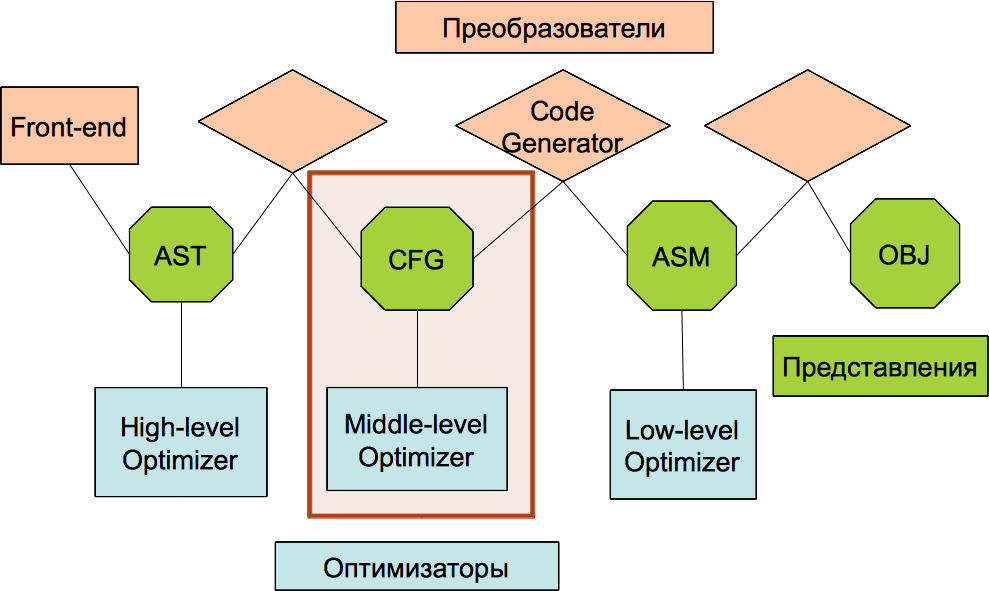
\includegraphics[width=140mm]{arch}}
        \caption{Архитектура оптимизирующего статического компилятора
                 \todo{перевести в вектор}}
        \label{fig:arch}
      \end{figure}

      Такой компилятор представляет из себя конвейер (рис. \ref{fig:arch}): на
      входе он получает исходный код программы, на выходе отдает бинарный код.
      Также существуют промежуточные представления, пригодные для работы
      оптимизаторов и необходимых им алгоритмов анализа.

      Для перевода программы из одного представления в другое существуют
      преобразователи.
      Самый первый преобразователь переводит исходный код или байт-код
      программы во внутреннее представление, с которым удобно работать другим
      компонентам компилятора.
      Последний преобразователь выполняет перевод в самое низкоуровневое,
      бинарное представление, содержащее данные и код, пригодный для исполнения
      на целевой архитектуре компилятора.

      \todo{картинку зависимостей между оптимизаторами и анализаторами}

      Оптимизации проводятся на одном из внутренних представлений, они
      модифицируют его с целью повышения эффективности исполнения программы
      относительно заданного критерия. Однако, эти преобразования должны быть
      корректными. Анализаторы предоставляют информацию о свойствах программы,
      и на основании этой информации определяется, можно ли
      проводить оптимизацию. Таким образом, анализаторы~--- это вспомогательные
      компоненты, необходимые для проведения корректных оптимизаций.

      Рассмотрим оптимизацию выноса инвариантов цикла (англ.
      \eng{loop-invariant code motion}) на примере \ref{code:licm}.
      Для выноса какого-либо выражения из цикла, требуется убедиться, что оно
      не будет изменяться (является инвариантом цикла).
      В данном примере, кандидатом на вынесение из цикла является выражение
      $x.field$. Оптимизатору необходимо убедиться, что поле объекта, на
      который ссылается переменная $x$ не изменяется при выполнении других
      инструкций тела цикла. В данном примере оптимизатору необходимо знать,
      могут ли переменные $x$ и $y$ быть синонимома. Если могут, то
      проводить оптимизацию нельзя, так как запись в $y.field$ может изменить
      значение $x.field$. Если же переменные точно не являются синонимами,
      проведение оптимизации корректно.

      \begin{algorithm}
        \caption{Вынесение инвариантов цикла}
        \label{code:licm}
        \begin{multicols*}{2}
          \algorithmictitle{Исходный код}
          \begin{algorithmic}[1]
            \FOR{$i = 1$ to \textbf{length}($a$)}
            \STATE $y.field = func(i)$
            \STATE $a[i] = x.field$
            \ENDFOR
          \end{algorithmic}
          \columnbreak
          \algorithmictitle{Преобразованный код}
          \begin{algorithmic}[1]
            \STATE $temp = x.field$
            \FOR{$i = 1$ to \textbf{length}($a$)}
            \STATE $y.field = func(i)$
            \STATE $a[i] = temp$
            \ENDFOR
          \end{algorithmic}
        \end{multicols*}
      \end{algorithm}

      Анализ синонимов описанный в работе позволяет отвечать на
      вопрос оптимизатора: «А могут ли две переменные ссылочного типа быть
      синонимами?»

    \subsection{Анализ многопоточных программ}

      Компьютеры, в которых несколько процессоров взаимодействуют с
      использованием разделяемой памяти, разрабатываются с 1960-х годов, а
      сейчас они уже распространены повсеместно. Изначально доступ к общей
      памяти был строго последовательным для всех потоков, исполнявшихся на
      разных процессорах. Но со временем появились весьма изощренные техники
      повышения производительности работы с общей памятью: многоуровневые кэши,
      внеочередное исполнение и другие. Это привело к тому, что взаимодействие
      с разделяемой памятью усложнилось с точки зрения программиста.

      Рассмотрим пример \ref{code:out_of_order_exec}, исполнение которого на
      современном процессоре может привести к неожиданному результату.
      Если изначально $obj.x = obj.y = 0$, то по окончанию работы примера
      значения переменных $x$ и $y$ могут равняться так же нулю. Это связано с
      тем, что процессор при исполнении первого потока мог сначала выполнить
      вторую инструкцию, так как она не зависит от первой, аналогично при
      исполнении второго потока.

      \begin{algorithm}
        \caption{Нарушение логики программы при внеочередном исполнении}
        \label{code:out_of_order_exec}
        \begin{multicols*}{2}
          \algorithmictitle{Поток 1}
          \begin{algorithmic}[1]
            \STATE $obj.x = 1$
            \STATE $y = obj.y$
          \end{algorithmic}
          \columnbreak
          \algorithmictitle{Поток 2}
          \begin{algorithmic}[1]
            \STATE $obj.y = 1$
            \STATE $x = obj.x$
          \end{algorithmic}
        \end{multicols*}
      \end{algorithm}


      При исполнении многопоточной программы на многопроцессорной машине,
      два последовательных чтения поля одного и того же объекта могут
      возвращать разные значения, так как в параллельном потоке могла произойти
      запись в это же поле в промежуток времени между последовательными
      чтениями. Если исходить из таких соображений, то анализ указателей
      получится черезчур консервативным: любое поле объекта может указывать
      хоть на что. Очевидно, что это не является приемлимым результатом.

      На самом деле в большинстве систем есть определенные правила,
      регулирующие работу с памятью. Такие правила есть на уровне процессора,
      виртуальной машины и языка. Эти правила называют моделью памяти,
      модель памяти для многопоточной системы определяет в каком
      порядке будут происходить доступы к памяти и, как следствие, какие
      значения может возвращать конкретное чтение памяти.


  %%%%%%%%%%%%%%%%%%%%%%%%%%%%%%%%%%%%%%%%%%%%%%%%
  %             Постановка задачи
  %%%%%%%%%%%%%%%%%%%%%%%%%%%%%%%%%%%%%%%%%%%%%%%%
  \section{Постановка задачи}

    Целью данной работы является изучение существующих алгоритмов анализа
    указателей, последующая разработка внутрипроцедурного алгоритма и
    внутренного представления для использования в оптимизирующем
    статическом компиляторе Java программ
    \eng{Excelsior Research Virtual Machine (Excelsior~RVM)}
    \cite{excelsior_jet} с учетом приведенных ниже требований.

    Алгоритм анализа должен учитывать следующие особенности языка Java:
    \begin{itemize}
      \item наличие строгой типизации,
      \item отсутствие адресной арифметики,
      \item отсутствие указателей на указатели.
    \end{itemize}
    Именно эти особенности отличают язык Java от языка C при рассмотрении
    анализа указателей, для которого были
    спроектированны классические алгоритмы анализа указателей
    Стинсгарда \cite{steensgaard} и Андерсена \cite{andersen}.

    В свзяи с широким распространением многопоточных программ,
    алгоритм анализа необходимо адаптировать для применения к
    многопоточным программам согласно спецификации JVM, которая имеет
    строгое и подробное описание модели памяти (Java Memory Model)
    \cite{manson_jmm}.

    Кроме того внутреннее представление программы должно быть адаптировано,
    для хранения результатов анализа указателей, и предоставлять удобный
    интерфейс для получения этих результатов другими алгоритмами статического
    анализа.

    Для достижения поставленной цели необходимо:
    \begin{itemize}
      \item изучив существующие алгоритмы анализа указателей, выбрать
            подходящий внутрипроцедурный алгоритм и адаптировать его
            для анализа многопоточных программ на языке Java,
      \item адаптировать существующее внутреннее представление программы для
            хранения результатов анализа указателей,
      \item реализовать алгоритм и внутреннее представление для оптимизирующего
            статического компилятора Java программ \eng{Excelsior RVM}.
    \end{itemize}

  %%%%%%%%%%%%%%%%%%%%%%%%%%%%%%%%%%%%%%%%%%%%%%%%
  % Описание алгоритма анализа
  %%%%%%%%%%%%%%%%%%%%%%%%%%%%%%%%%%%%%%%%%%%%%%%%
  \section{Описание алгоритма анализа}
    \label{section:algorithm}

    \subsection{Строгая система типов языка Java}
    \label{section:type_system}

      \todo{Паша сказал, что тут написан бред, поправить.}
      \remark{Как? Нужно дать нормальное определение, или просто убрать
      про примитивные типы?}

      Так как до сих пор нет устоявшегося определения строгой типизации
      \todocite, для определенности рассмотрим строгую систему типов языка
      Java.

      В Java ссылочными типами являются классы, интерфейсы, массивы других
      типов; примитивные типы можно не рассматривать в контексте анализа
      указателей, так как они не могут переносить информацию о целях
      указателей. Все классы и массивы являются наследниками типа
      $java\-.lang\-.Object$ (далее просто $Object$), будем считать,
      не ограничивая общность, что все интерфейсы также являются
      наследниками типа $Object$.

      В Java допускается присваивание переменной только значения, имеющего
      такой тип данных, что существует расширяющее преобразование к типу этой
      переменной.
      Например, преобразование типа byte к типу int, преобразование ссылочного
      типа к его предку являются расширяющими преобразованиями, они безопасны и
      не требуют дополнительных действий на этапе исполнения.
      А преобразование типа double к типу float, преобразование типа $Object$ к
      другому ссылочному типу являются сужающими, могут приводить к потере
      данных и требуют проверок на этапе исполнения.

    \subsection{Внутреннее представление и SSA-форма программы}
      \label{section:ir_and_ssa}

      В процессе компиляции программа на исходном языке программирования
      переводится в, так называемое, внутреннее представление программы
      (англ. \eng{internal representation, IR}), на котором работают
      алгоритмы анализа и на котором проводятся все оптимизации.
      Рассмотрим внутреннее представление тела функции, заданное в виде
      графа управления (англ. \eng{control flow graph, CFG}), именно это
      внутреннее представление используется для проведения большинства
      оптимизаций в современных компиляторах \todocite.
      CFG~--- это ориентированный граф, в котором вершинам соответствуют
      последовательности операторов программы, а дугам~--- переходы из конца
      одной последовательности операторов в начало другой. Такие
      последовательности операторов, являющиеся вершинами, назовем линейными
      участками. В конце каждого линейного участка присутствует оператор
      перехода, который передает управление по одной из дуг, выходящих из
      данной вершины CFG.

      Будем говорить, что программа находится в SSA-форме (\eng{Static Single
      Assignment}), если существует не более одного присваивания каждой
      переменной. В SSA-форме вводится дополнительная операция слияния значений
      переменных, так называемая $\phi$-функция. Пусть в CFG программы
      существует вершина $N$, такая что в нее входит больше одной дуги из
      вершин $N_1$, ..., $N_K$, назовем такую вершину точкой слияния. Тогда в
      $N$ будут располагаться следующие вызовы $\phi$-функций
      \[ v = \phi(v_1, ..., v_K), \]
      для всех переменных $v$ требующих слияния.
      Семантика данной операции заключается в присваивании переменной $v$
      значения переменной $v_i$, соответствующего вершине $N_i$, из которой
      управление пришло в $N$. В случае CFG, приведенного на рисунке
      \ref{fig:cfg_with_phi}, переменной $a_3$ будет присвоено значение 5 или
      7, если управление придет в нижнюю вершину через левую или правую
      вершину, соответственно.

      \begin{figure}[!htb]
        \center{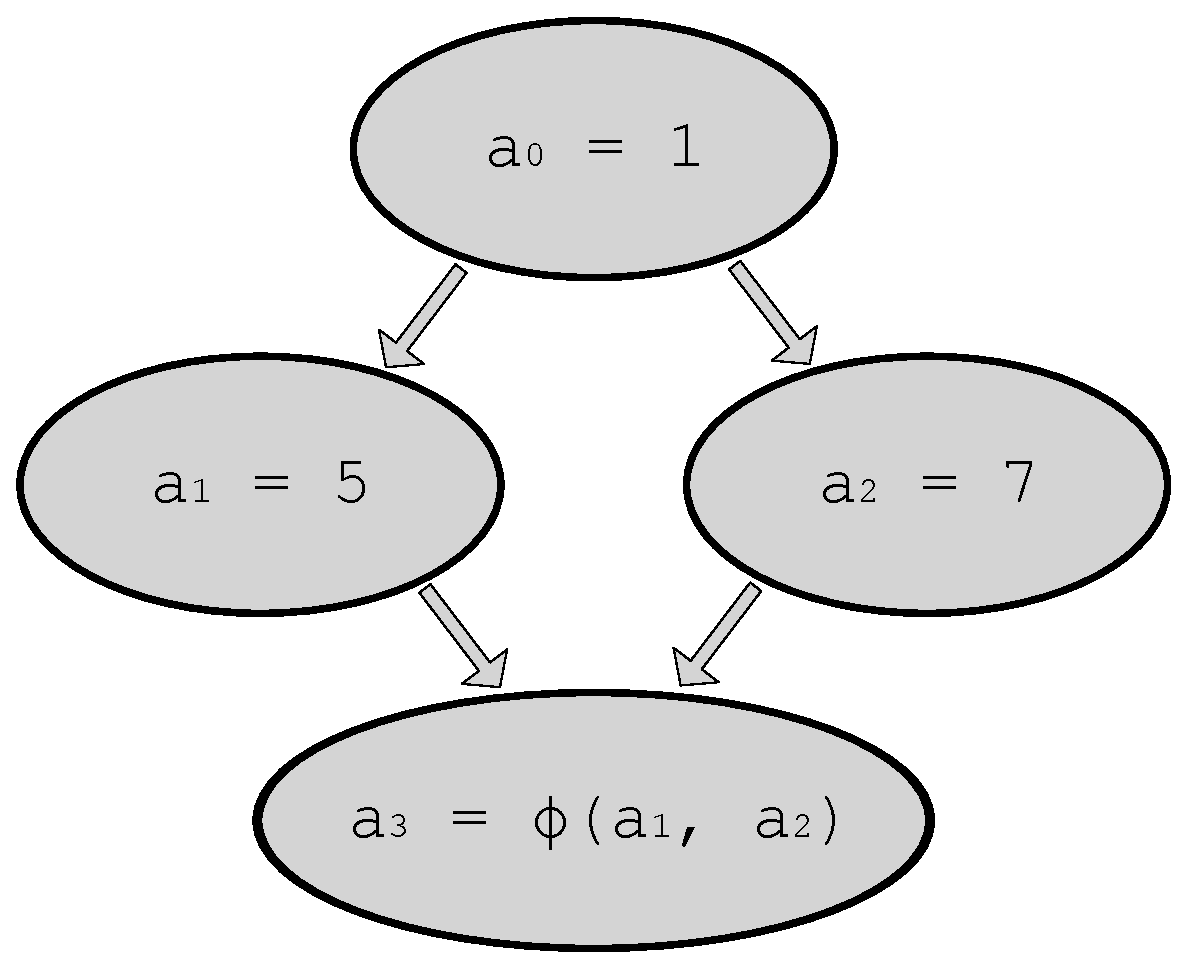
\includegraphics[width=160mm]{phi_func}}
        \caption{Пример CFG в SSA-форме с $\phi$-функцией}
        \label{fig:cfg_with_phi}
      \end{figure}

      Для преобразования программы в SSA-форму и обратно существуют эффективные
      алгоритмы \cite{ssa}. В то же время
      многие виды анализа и многие оптимизации проще и эффективнее проводить
      именно на программе в SSA-форме, поэтому ее и
      будем использовать для проведения анализа указателей.

    \subsection{Операции и их семантика}
      \label{section:instructions}

      Сначала определим точно, что может быть указателем в языке Java и
      подобных ему.

      В отличии от C-подобных языков, где допустимы указатели на:
      \begin{itemize}
        \item объекты в куче,
        \item объекты на стеке,
        \item другие переменные,
        \item функции;
      \end{itemize}
      в Java-подобных языках целью
      указателя может быть только объект, находящийся в куче. Так же
      отсутствует адресная арифметика (операции взятия адреса,
      чтения и записи по адресу), за счет чего ссылка на объект может
      появиться только явно, по цепочке присваиваиний, начиная с создания этого
      объекта в куче.

      При проведении анализа указателей достаточно учитывать не все операции
      допустимые в языке, а лишь те, которые могут изменять цели указателей.
      Достаточно рассматривать следующие инструкции ($a$, $b$, $c$~---
      переменные или формальные параметры ссылочного типа):
      \begin{table}
        \begin{tabular}{|l|p{120mm}|}\hline
          \textbf{Инструкция} & \textbf{Описание}\\ \hline

          $a = b$
          & присваивание значения $b$ переменной $a$ \\ \hline

          $a = \NULL$
          & указание, что $a$ не указывает ни на один объект \\ \hline

          $a = \NEW T$
          & создание нового объекта типа $T$ в куче \\ \hline

          $a = b.f$
          & чтение поля объекта, на который ссылается $b$ \\ \hline

          $b.f = a$
          & запись в поле объекта, на который ссылается $b$ \\ \hline

          $a = T.f$
          & чтение статического поля класса $T$ \\ \hline

          $T.f = a$
          & запись в статическое поле класса $T$ \\ \hline

          $a = b$[\ldots]
          & чтение элемента массива $b$ \\ \hline

          $b[\ldots] = a$
          & запись в элемент массива $b$ \\ \hline

          $a = (T)b$
          & преобразования значения переменной $b$ к типу $T$ \\ \hline

          $a = \textrm{foo}(b, \ldots)$
          & вызов функции foo, возращающей значение ссылочного типа \\ \hline

          $\textrm{foo}(b, \ldots)$
          & вызов функции foo, либо не возращающей значение, либо возвращающей значение примитивного типа \\ \hline
        \end{tabular}
        \caption{Инструкции влияющие на цели указателей}
        \label{tabular:instructions}
      \end{table}

      Рассмотрим чтение и запись элементов массива подробнее. Зачастую
      алгоритм анализа не может определить реальных значений индексов
      элементов, по которым происходит доступ к элементам массива, так как их
      значения будут доступны лишь во время исполнения программы. По этой
      причине алгоритм анализа не может различать доступ к отдельным элементам
      массива, мы вынуждены поступать консервативно: рассматривать все элементы
      массива как единый элемент, из которого читаются и в который записываются
      все значения при обращении к любому элементу.

      При преобразовании $a$ = ($T$)$b$ в случае неудачного преобразования
      значения переменной $b$ к типу $T$ будет выброшено исключение во время
      исполнения, поэтому в рамках анализа, можно считать что переменная $a$
      может указывать только на объекты, совместимые по присваиванию с типом
      $T$.

      При вызове другой функции нужно понимать, что вызванная функция может
      изменять цели полей переданных параметров и полей статических переменных.


    \subsection{Тип алгоритма}

      Необходимо определиться с характеристиками алгоритма анализа
      подходящего для нашей задачи. Описание основных характеристик уже было
      приведено в разделе~\ref{section:analysis_overview}.

    \subsubsection{\eng{Subset-based} алгоритм анализа}

      При выборе между \eng{subset-based} и \eng{equality-based} алгоритмами
      анализа, необходимо решить, что важнее в конкретном случа:
      точность или скорость работы, соответственно.
      Хотя время работы \eng{subset-based} алгоритма кубически зависит от
      размеров программы, а для \eng{equality-based} практически линейно,
      проведенные эксперименты показывают \cite{shapiro_fast_and_accurate}, что
      на небольших программах (до 3000 строк), время работы обоих алгоритмов
      анализа примерно одинаково, но точность у \eng{subset-based} алгоритма
      значительно выше.
      Забегая вперед, отметим, что алгоритм будет применятся для
      внутрепроцедурного анализа, и поэтому, выбирая \eng{subset-based}
      алгоритм, выигрыш в точности анализа будет весомым, а потери во времени
      работы алгоритма незначительны, так как отдельный метод программы
      разумно отнести к «небольшим программам».

    \subsubsection{Нечувствительный к потоку алгоритм анализа}
      \label{section:flow_sensetive_analysis}

      Рассмотрим другую характеристику алгоритма анализа указателей:
      чувствительность к потоку управления в программе.
      Если алгоритм анализа чувствителен к потоку управления, то результатом
      его работы являются наборы целей указателей для конкретных точек
      программы.
      Хотя объем этих результатов, при простейшем подходе, увеличивается
      пропорционально количеству инструкций программы, что приводит к
      дополнительному потреблению памяти, такой алгоритм дает более точные
      результаты \cite[с.~57]{hind_pointer_analysis_not_solved_yet}.

      Напомним, что точность чувствительного к потоку анализа обусловлена
      использованием строгих присваиваний (англ. \eng{strong update}).
      Строгое присваивание в отличии от обычного присваивания по возможности
      заменяет текущий набор целей указателя на новый, а не расширяет его.
      Однако известно, что эффекта строгого присваивания для переменных
      верхнего уровня можно добиться, переведя программу в SSA-форму
      \cite{points_to_with_efficient_strong_updates}.

      Продемонстрируем работу нечувствительного к потоку алгоритма на примере
      \ref{code:ssa_precision} (это пример \ref{code:control_flow} переведенный
      в SSA-форму).
      \begin{algorithm}
        \caption{Повышение точности за счет использования SSA-формы}
        \label{code:ssa_precision}
        \begin{algorithmic}[1]
          \REQUIRE $x_0$, $x_1$, ..., $x_i$~--- версии одной переменной $x$
          \STATE $a_0$ = \NEW T()
          \STATE $b_0$ = \NEW T()
          \STATE $c_0$ = \NEW T()
          \STATE $a_1$ = $b_0$
          \STATE $b_1$ = $c_0$
          \STATE $c_1$ = $a_1$
        \end{algorithmic}
      \end{algorithm}

      Так как присутствует только одно присваивание каждой переменной, легко
      получается следующий результат:
      \[Pts(a_0) = \{O_a\}, Pts(b_0) = \{O_b\}, Pts(c_0) = \{O_c\},\]
      \[Pts(a_1) = \{O_b\}, Pts(b_1) = \{O_c\}, Pts(c_1) = \{O_b\}.\]
      Как было показано в разделе \ref{section:analysis_overview}
      чувствительный к
      потоку алгоритм анализа дает идентичный результат для конечной точки
      примера \ref{code:control_flow} (учитывая, что для конечной точки
      программы $a = a_1$, $b = b_1$, $c = c_1$):
      \[Pts(a) = \{O_b\}, Pts(b) = \{O_c\}, Pts(c) = \{O_b\}.\]

      \todo{Паша, таки какой будем использовать? Ибо доводов за
      нечувствительный не остается}
      %В итоге получается, что чувствительный к потоку алгоритм и алгоритм
      %анализа, работающий на SSA-форме программы, дают
      %одинаково точные результаты и каждый требует дополнительной памяти, либо
      %на хранение набора целей указателей для точек программы, либо на хранение
      %целей указателей для всех версий переменной. Но необходимо заметить, что
      %большинство современных компиляторов, и \eng{Excelsior RVM} в том числе,
      %уже используют SSA-форму для программы, и следовательно, при прочих
      %равных нет смысла использовать чувствительный к потоку алгоритм анализа.

    \subsubsection{Внутрипроцедурный алгоритм анализа}

      Хотя межпроцедурные алгоритмы анализа указателей и дают более точные
      результаты, они сложны для реализации, тем более для таких
      языков как Java, где каждый нестатический метод является виртуальным.
      Реализация такого алгоритма анализа выходит за рамки моей
      квалификационной работы, в ней рассматриваются внутрепроцедурные
      алгоритмы. Однако отсутствие межпроцедурного анализа смягчается, так
      как до вызова алгоритма анализа указателей может быть проведена
      оптимизация открытой подстановки методов.

    \subsection{Описание алгоритма анализа для однопоточных программ}

      В этом разделе будет приведено описание алгоритма анализа указателей
      для однопоточных Java программ.
      Представленный алгоритм является внутрипроцедурным алгоритмом
      \eng{subset-based} типа нечувствительного к потоку управления,
      работающим с программой в SSA-форме.

      Заметим, что для однопоточной программы статические поля классов можно
      рассматривать как глобальные переменные.

      При анализе отдельно взятого метода каждой переменной ссылочного типа
      ставится в соответствие множество ее целей. Для локальных переменных
      это множество изначально пустно. Для формальных параметров и глобальных
      переменных необходимо сделать консервативное предположение, что две любых

      переменных из формальных параметров и глобальных переменных могут быть
      синонимами. Этого можно добиться, если их множество будет содержать один
      специальный объект $O_{unknown}$ искусственного типа $Unknown$ такого,
      что существует расширяющее преобразование этого типа к любому другому
      ссылочному типу.

      У любого объекта, у которого есть поля, так же хранится множестве целей
      каждого из них. У объекта $O_{unknown}$ существует единственное поле
      $field$ типа $Object$, и доступ к любым полям объекта $O_{unknown}$
      транслируется в доступ к полю $field$. Изначально множество целей
      поля $field$ объекта $O_{unknown}$ содержит один объект~---
      $O_{unknown}$.

      Введем следующие обозначения
      \begin{eqnarray*}
        \textrm{множество целей переменной $a$}&:& \VPts{a}, \\
        \textrm{множество целей поля $f$ объекта $O$}&:& \OFPts{O}{f}.
      \end{eqnarray*}
      Можно определить цели поля $f$ переменной $a$ следующим образом
      \[ \bigcup\limits_{O \in \VPts{a}} \OFPts{O}{f}.\]
      Определим, как инструкции, описанные в разделе \ref{section:instructions}
      изменяет множество целей переменных и полей объектов.

      Присваивание $a = b$ просто расширяет множество целей переменной $a$
      \[\VPts{a} = \VPts{a} \cup \VPts{b},\]
      присваивание $a = \NULL$ не изменяет множество целей переменной $a$.

      Присвание $a = b.f$ нужно трактовать как множество присваиваний
      переменной $a$ значений полей объектов, на которые может указывать переменная
      $b$:
      \[
        \textbf{for } O \textbf{ in } \VPts{b} \colon
        \; \VPts{a} = \VPts{a} \cup \OFPts{O}{f}.
      \]
      Присвание $b.f = a$ похоже на предыдущее. Его нужно трактовать как
      множество присваиваний полей объектов, на которые может указывать
      переменная $b$, значению переменной $a$:
      \[
        \textbf{for } O \textbf{ in } \VPts{b} \colon
        \; \OFPts{O}{f} = \OFPts{O}{f} \cup \VPts{a}.
      \]

      При преобразовании значения переменной к некоторому типу $T$
      ($a = (T)b$), необходимо расширить множество целей переменной $a$ только
      объектами, совместимыми по присваиванию с типом $T$. Для этого необходимо
      хранить формальный тип объекта, зная его, можно определить совместимость
      по присваиванию ($\IsAssignable{O}{T}$) для некоторого объекта $O$ и
      ссылочного типа $T$\remark{ (нужно ли это описывать?)}.
      Тогда для обработки такого преобразования нужно следующее действие:
      \[
        \VPts{a} = \VPts{a} \cup
            \left\{ O \colon O \in \VPts{b}, \IsAssignable{O}{T} \right\}.
      \]

      Для обработки присваивания нового объекта переменной, занумеруем
      все места создания объектов в методе. Тогда присваивание $a = \NEWi{i} T$
      приводит к добавлению в $\VPts{a}$ объекта $O_i$, уникального
      объекта связанного с $i$-ым местом создания объекта.

      При передачи ссылочных переменных в качестве параметров в другие
      методы необходимо поступать консервативно, так как вызываемый метод
      может произвольным способом изменять поля объектов, на которые прямо или
      косвенно ссылаются переданные параметры и глобальные паременные. Поэтому
      если некоторая переменная $b$ передается в другой метод необходимо
      сделать следующее:
      \todo{заменить VPts на список всех-всех утекающих объектов}
      \begin{eqnarray*}
        &&\textbf{for } O \textbf{ in } \VPts{b} \colon \\
        &&\quad\textbf{for } f \textbf{ in fields of } O \colon \\
        &&\qquad\OFPts{O}{f} = \OFPts{O}{f} \cup \{O_{unknown}\}.
      \end{eqnarray*}
      Возвращаемое значение метода так же консервативно полагается равным
      $O_{unknown}$.

    \subsection{Модель памяти языка Java}

      В этом разделе описана модель памяти представленная в спецификации языка
      Java версии 5.0. Она, в частности, задает, какое поведение многопоточных
      программ является корректным, и указывает, какие преобразования программ
      допустимы в виртуальных машинах и компиляторах.

      Модели памяти различаются по тому, насколько сильные ограничения
      накладываются на последовательность исполнения инструкций чтения и
      записи.
      Модель памяти может быть очень строгой и требовать
      последовательного исполнения всех инструкций чтения и записи.
      Такая модель сильно ограничивает набор используемых оптимизаций,
      так как многим из них требуется менять отдельные инструкции чтения и
      записи местами, а строгая модель памяти не позволит это сделать, даже
      если между инструкциями нет зависимости по управлению и данным.
      Слабая модель памяти может не определять какого-либо жесткого порядка
      исполнения инструкций. Основываясь на этой модели компилятор может
      довольно сильно преобразовывать программу с целью ее оптимизации,
      однако разработчику этой программы придется уделять очень много времени
      для написаная корректной программы в рамках такой слабой модели памяти.

      Модель памяти представленная в спецификации языка Java версии 5.0 является
      компромиссом между возможностью проведения широкого класса оптимизаций и
      удобством разработки программ на языке Java. Подробное описание можно
      найти в спецификации JSR-133 \cite{jsr133}. Модель памяти является
      достаточно строгой и однозначно определяет, как будут исполняться
      корректно синхронизованные программы (программы в которых отсутствуют
      состояния гонки (англ. \eng{data-race-free programs})). Однако она
      является и достаточно слабой, позволяя проводить многие оптимизации.

      Рассмотрим подробнее семантику чтения и записи полей с учетом данной
      модели памяти (подробнее в \cite{jsr133_cookbook}).

      Сначала определим, какие инструкции чтения или записи памяти разрешено
      переставлять компилятору. Ему позволяется переставлять две инструкции
      чтения или записи обычных полей, если между ними нет зависимости по
      данным. Но не позволяется переставлять две инструкции чтения или записи
      \eng{volatile} полей. Так же не позволяется переставлять две инструкции,
      где первая~--- чтение или запись обычного поля, а вторая~--- запись в
      \eng{volatile} поле, или где первая~--- чтение \eng{volatile} поля, а
      вторая~--- чтение или запись обычного поля.

      Далее определим, какие значения могут возвращать чтения разделяемой
      памяти. Модель памяти гарантирует, что после записи значения в
      \eng{volatile} поле одним из потоков, все последующие чтения этого
      поля вернут новое значение. Но подобное поведение не гарантируется
      при работе с обычными полями. Запись в обычное поле одним из потоков
      может быть не видна другим потокам при чтении этого поля. Это может
      происходить из-за наличия у каждого потока локальных копий обычных полей.
      Однако модель памяти определяет, когда эти локальные копии обязаны быть
      синхронизованны с реальной разделяемой памятью: при записи в
      \eng{volatile} поле все локальные записи памяти должны быть отражены
      в разделяемой памяти, а при чтении \eng{volatile} поля все локальные
      данные должны быть заново прочитаны из разделяемой памяти.

      Данные правила можно пояснить на примере \ref{code:volatile_synch}.
      В первом потоке запись данных произойдет до установки флага готовности,
      так он является \eng{volatile}, и следовательно не может быть переставлен
      с предыдущей инструкцией. Так же при установке флага готовности данные
      гарантированно будут записаны в разделяемую память.
      Во втором потоке после чтения \eng{volatile} флага данные будут прочитаны
      именно из разделяемой памяти, причем это произойдет после чтения флага,
      так как эти две операции не могут быть переставлены.
      Следовательно, если данные будут выставлены первым потоком, то именно
      они и будут прочитаны вторым потоком.
      \begin{algorithm}
        \caption{Синхронизация через \eng{volatile} переменную
          ($data$~--- обычное поле, $ready$~--- \eng{volatile} поле)}
        \label{code:volatile_synch}
        \begin{multicols*}{2}
          \algorithmictitle{Поток 1}
          \begin{algorithmic}[1]
            \STATE $data$ = get\_data()
            \STATE $ready$ = \BOOLTRUE
          \end{algorithmic}
          \columnbreak
          \algorithmictitle{Поток 2}
          \begin{algorithmic}[1]
            \WHILE{ \textbf{not } $ready$ }
            \STATE \COMMENT{waiting}
            \ENDWHILE
            \STATE use\_data($data$)
          \end{algorithmic}
        \end{multicols*}
      \end{algorithm}

      Отдельно стоит сказать про \eng{final} поля классов и объектов.
      В языке Java до версии 5.0 \eng{final} поля могли изменять свое значение
      при определенных условиях. Однако представленная модель памяти
      гарантирует, что \eng{final} поля не будут изменяться во время
      исполнения. Соответственно, единожды прочитанное значение \eng{final}
      поля можно сохранить, и при последующих чтениях этого поля возвращать
      сохраненное значение.
      Заметим, что для конструкторов, в которых происходят изначальные
      присваивания в \eng{final} поля, подобных гарантий о неизменности
      \eng{final} полей нет по понятным причинам.

      В данном разделе не описывались инструкции виртуальной Java машины
      monitorenter и monitorexit, так они дают эффект идентичный,
      соответственно, чтению и записи \eng{volatile} полей.

    \subsection{Описание алгоритма анализа для многопоточных программ}

      Описанные в предыдущем разделе свойства модели памяти языка Java версии
      5.0 необходимо учесть при адаптации алгоритма для анализа многопоточных
      программ.

  %%%%%%%%%%%%%%%%%%%%%%%%%%%%%%%%%%%%%%%%%%%%%%%%
  % Архитектура системы
  %%%%%%%%%%%%%%%%%%%%%%%%%%%%%%%%%%%%%%%%%%%%%%%%
  \section{Архитектура системы}

    \subsection{Архитектура оптимизирующего компилятора}

      \todo{убрать, ибо общая архитектура описана в описании предметной
      области}

      Рассмотрим общую архитектуру оптимизирующего статического компилятора,
      в который необходимо интегрировать описанный в разделе
      \ref{section:algorithm} алгоритм анализа.

      \begin{figure}[!htb]
        \center{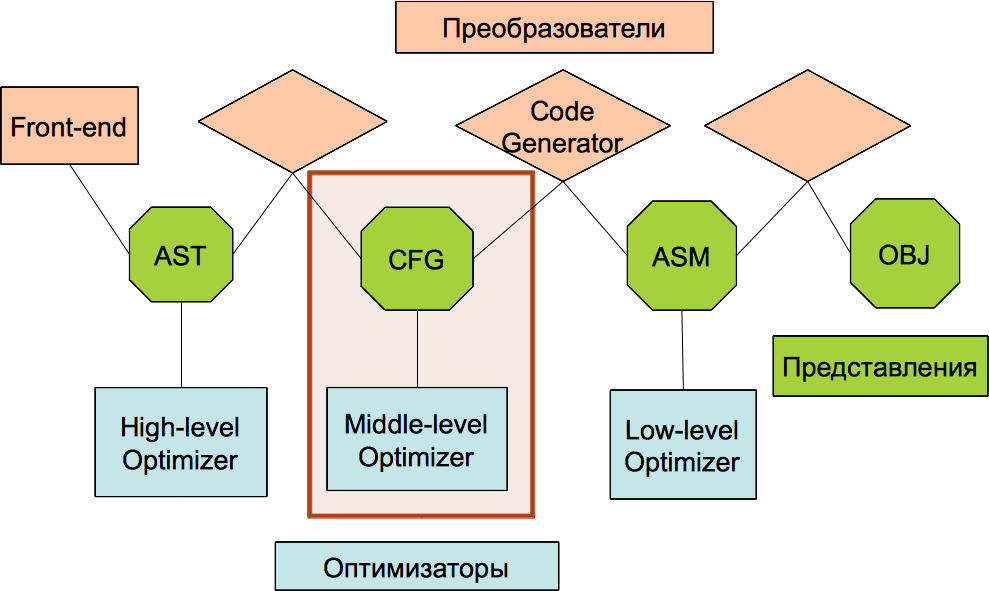
\includegraphics[width=140mm]{arch}}
        \caption{Архитектура оптимизирующего статического компилятора
                 \todo{перевести в вектор}}
        \label{fig:arch2}
      \end{figure}

      Такой компилятор представляет из себя конвейер: на входе он получает
      исходный код программы, на выходе отдает бинарный код. Также существуют
      промежуточные представления, пригодные для работы оптимизаторов и
      необходимых им алгоритмов анализа.

      Для перевода программы из одного представления в другое существуют
      преобразователи.
      Самый первый преобразователь переводит исходный код или байт-код
      программы во внутреннее представление, с которым удобно работать другим
      компонентам компилятора.
      Последний преобразователь выполняет перевод в самое низкоуровневое,
      бинарное представление, содержащее данные и код, пригодный для исполнения
      на целевой архитектуре компилятора.

      \todo{картинку зависимостей между оптимизаторами и анализаторами}

      Большинство оптимизаций, которым требуются результаты анализа указателей,
      проводятся на среднем уровне (\eng{Middle-level optimizer}), который
      работает с внутренним представлением в виде CFG (это верно для
      большинства современных оптимизирующих компиляторов, для Excelsior RVM в
      том числе). Разработанная компонента для проведения анализа указателей
      будет располагаться на этом же уровне и использовать то же внутреннее
      представление.

    \subsection{Компонента, выполняющая анализ синонимов}
      \label{section:analysis_component}

      Типичное использование анализа синонимов оптимизаторами сводится к
      последовательности запросов о том, могут ли пары переменных быть
      синонимами.
      Компонента, выполняющая анализ синонимов и способная отвечать на подобные
      запросы, реализована в виде отдельного класса, с двумя публичными
      методами.
      Первый метод, конструктор, принимает ссылку на один из методов программы.
      Второй метод проводит анализ синонимов для двух данных переменных метода
      и возвращает, могут ли они быть синонимами.

  %%%%%%%%%%%%%%%%%%%%%%%%%%%%%%%%%%%%%%%%%%%%%%%%
  % Реализация
  %%%%%%%%%%%%%%%%%%%%%%%%%%%%%%%%%%%%%%%%%%%%%%%%
  \section{Реализация}

    Изначально был реализован тестовый стенд, изолированное окружение для
    проведения экспериментов. С его помощью можно проверять работу
    разных алгоритмов анализа указателей на характерных примерах, сравнивать их
    характеристики. Изолированность позволяет быстро разработать такую систему
    и легко вносить в нее изменения, так как не требуется интеграция с
    существующими интерфейсами оптимизирующего компилятора.

    \subsection{Реализация тестового стенда}

      Реализована система, являющаяся простой моделью компилятора. Она включает
      в себя парсер простого Java-подобного языка, структуру для хранения
      внутреннего представления и компоненту, выполняющую анализ указателей.
      Так же присутствуют методы просмотра разнообразной статистики: множества
      целей всех указателей присутствующих в программе, точности результатов,
      времени работы алгоритма.

      Система принимает на входе программу в специальном формате через
      стандартный поток ввода. В начале программы идут определения классов в
      стиле Java с поддержкой наследования, статических и обычных полей. Затем
      задается тело метода, для которого и будет проводится анализ указателей.
      Для метода указывается список формальных параметров и его тело в
      SSA-форме в виде CFG, на каждом линейном участке которого присутствуют
      только операции из таблицы \ref{tabular:instructions}.

      Парсер на выходе получает AST (\eng{Abstract Syntax Tree}), из которого
      инициализируется иерархия классов и CFG единственного метода, который
      передается в анализатор для проведения анализа указателей. Анализ
      проводится с помощью тестируемого алгоритма. На выходе предоставляются
      результаты в виде наборов целей указателей и
      другая статистика работы алгоритма.

      Система реализована на языке Ruby, так как он позволяет очень быстро
      создать работающее приложение, для которого скорость работы не является
      критической характеристикой. Парсер осуществляет разбор входной
      программы с использованием регулярных выражений, что так же является
      простым и быстрым в исполнении решением. Внутреннее представление метода
      реализовано в виде двусвязного графа линейных участков программы,
      которые состоят из последовательности операций. При инициализации этого
      внутреннего представления проверяется корректность графа и всех операций.

      Парсер и модуль инициализации внутреннего представления имеют хорошее
      покрытие модульными тестами (англ. \eng{unit test}). Разные варианты
      алгоритма анализа указателей также имеют модульные тесты для тестирования
      особенностей конкретного алгоритма.

    %\subsection{Конечная компонента анализа}

    %  Компонента описанная в разделе \ref{section:analysis_component}
    %  реализована в виде отдельного класса. В конструкторе сохраняется
    %  ссылка на анализируемый метод, а анализ синонимов проводится следующим
    %  образом: сначала запускается алгоритм анализа указателей описанный в
    %  разделе \ref{section:algorithm} для CFG указанного метода, и на основе
    %  полученных результатов о целях переменных возвращается результат, могут
    %  ли данные переменные быть синонимами.

    %  Дополнительного применяется кэширование результатов, так как известно,
    %  что запросы о синонимичности переменных одного и того же метода
    %  повторяются многократно:
    %  при повторном запросе анализа синонимов, анализ указателей проводится
    %  только если CFG данного метода изменялся \todo{(как именно получается эта
    %  информация)}.

  %%%%%%%%%%%%%%%%%%%%%%%%%%%%%%%%%%%%%%%%%%%%%%%%
  % Практические результаты
  %%%%%%%%%%%%%%%%%%%%%%%%%%%%%%%%%%%%%%%%%%%%%%%%
  \section{Практические результаты}

    Представленный алгоритм анализа был реализован в рамках статического
    Java компилятора Excelsior RVM и протестирован на стандартных тестах
    производительности Java программ.
    В качестве набора тестов был взят SPECjvm2008 \cite{spec_jvm}, состоящий из
    реальных приложений и бенчмарков.

    При тестировании сравнивалась точность и скорость работы различных вариаций
    алгоритма анализа синонимов:
    \begin{itemize}
      \item алгоритм анализа не адаптированный для многопоточных программ;
      \item алгоритм анализа адаптированный для многопоточных программ;
      \item алгоритм анализа адаптированный для многопоточных программ с
            учетом семантики final полей.
    \end{itemize}
    Для сравнения так же тестировался простой алгоритм анализа указателей
    основанный на типах, описанный в \cite{diwan_tbaa}.

    Поскольку данные алгоритмы анализа являются заведомо корректными, имеет
    смысл сравнивать только их точность. В качестве метрики для сравнения
    точности использовалось усредненное количество синонимов для переменных
    ссылочного типа, появляющихся в программе: чем меньше это количество, тем
    выше точность. Такая метрика проста в реализации и удовлетворительна для
    языков со строгой типизацией, таких как Java
    \cite{hind_pointer_analysis_not_solved_yet}.

    Результаты тестирования приведены в таблице XX.
    \todo{таблица}

    \todo{Анализ результатов}

    Например: видно, что точность такого-то алгоритма горазде ниже чем точность
    других ...

    Но зато скорость ...

    И точность важнее ...

  %%%%%%%%%%%%%%%%%%%%%%%%%%%%%%%%%%%%%%%%%%%%%%%%
  % Заключение
  %%%%%%%%%%%%%%%%%%%%%%%%%%%%%%%%%%%%%%%%%%%%%%%%
  \sectionwithoutnumber{Заключение}

    Целью данной работы являлась разработка внутрипроцедурного алгоритма
    анализа указателей, адаптированного для анализа многопточных Java программ.
    Данная цель была успешно достигнута и в результате проведенной работы было
    сделано следующее:
    \begin{itemize}
      \item Проведен анализ существующих алгоритмов анализа указателей и
            синонимов, выделены их основные отличительные характеристики.
      \item Изучена спецификация модели памяти языка Java, выявлены свойства,
            влияющие на анализ указателей.
      \item Разработан внутрипроцедурный алгоритм анализа указателей,
            учитывающий особенности языка Java и адаптированный для анализа
            многопоточных программ в соответствии с моделью памяти языка Java.
      \item Разработано оптимальное внутреннее представление для хранения
            результатов анализа, являющееся компромиссом между объемом данных
            и скоростью доступа к ним.
      \item Реализован тестовый стенд для изучения свойств разных алгоритмов
            анализа указателей.
      \item Реализована компонента, интегрируемая в статический Java компилятор
            Excelsior RVM, выполняющая анализ синонимов.
      \item Проведено сравнение практических результатов работы разработанного
            алгоритма анализа с результатами других алгоритмов.
    \end{itemize}

    В дальнейшем планируется развитие представленного алгоритма: его адаптация
    для межпроцедурного анализа.
    Так же планируется реализация данного алгоритма анализа указателей и
    синонимов в промышленном статическом Java компиляторе Excelsior JET.

  %%%%%%%%%%%%%%%%%%%%%%%%%%%%%%%%%%%%%%%%%%%%%%%%
  %             Список литературы
  %%%%%%%%%%%%%%%%%%%%%%%%%%%%%%%%%%%%%%%%%%%%%%%%
  \newpage
  \addcontentsline{toc}{section}{Список литературы}
  %\begin{flushleft}
    \bibliography{../../biblio}
  %\end{flushleft}

  %%%%%%%%%%%%%%%%%%%%%%%%%%%%%%%%%%%%%%%%%%%%%%%%
  %               План график
  %%%%%%%%%%%%%%%%%%%%%%%%%%%%%%%%%%%%%%%%%%%%%%%%
  \newpage
  \thispagestyle{empty}
  \pagestyle{empty}
  \section*{План-график}

    \begin{center}
      \begin{tabular}{|p{10.5cm}|c|c|}\hline
        \textbf{Задача}                       &\textbf{Время} & \textbf{Срок}\\
        \hline
        Ознакомление с методами оптимизирующей компиляции, изучение
        основных понятий (SSA-форма внутреннего представления,
        виды статического анализа)
                                              & 2 недели    & 15 октября \\
        \hline
        Изучение работ по анализу указателей и синонимов для Си-подобных языков
                                              & 3 недели    & 10 ноября \\
        \hline
        Изучение спецификации Java Virtual Machine, системы типов языка Java;
        изучение работ по анализу указателей и синонимов для языка Java
                                              & 3 недели    & 30 ноября \\
        \hline
        Реализация тестовой модели и простейшего алгоритма, выполняющего
        анализ указателей для линейного участка программы
                                              & 3 недели    & 20 декабря \\
        \hline
        Реализация алгоритма, выполняющего внутрипроцедурный анализ для
        однопоточных Java программ, в рамках тестовой модели
                                              & 3 недели    & 31 января \\
        \hline
        Изучение спецификации Java Memory Model
                                              & 1 месяц     & 28 февраля \\
        \hline
        Преобразование алгоритма для анализа многопоточных Java программ
                                              & 1 месяц     & 31 марта \\
        \hline
        Интеграция созданного алгоритма в Java компилятор Excelsior RVM,
        тестирование корректности, быстродействия, точности и
        других характеристик
                                              & 1,5 месяца  & 15 мая \\
        \hline
      \end{tabular}
    \end{center}



  %%%%%%%%%%%%%%%%%%%%%%%%%%%%%%%%%%%%%%%%%%%%%%%%
  %                  Оценки
  %%%%%%%%%%%%%%%%%%%%%%%%%%%%%%%%%%%%%%%%%%%%%%%%
  \newpage
  \thispagestyle{empty}
  \pagestyle{empty}
  \section*{Оценка за апрельский отчёт}

    Руководитель: \underscore{1cm} (из 10 баллов).
    Подпись: \underscore{3cm} (Павлов\,П.\,Е.)

    \vspace{0.5cm}
    Преподаватель: \underscore{1cm}
\end{document}

